\chapter{Introduction to ordinal numbers with the Coq proof assistant}

\centerline{\LARGE {\bf work in progress!}}


The proof of termination of all hydra battles presented in~\cite{KP82} is based
on \emph{ordinal numbers}.
From a mathematical point of view, an ordinal is a representant of an equivalence class for isomorphims of strict, total and well-founded ordered sets.

\section{The mathematical point of view}

\subsection{Well-ordered sets}
Let us start with some definitions.
A  \emph{well-ordered set} is a set provided with a binary relation $<$ which has the following properties.
\begin{description}
\item[irreflexivity] : $\forall x\in A, x\not< x$
\item[transitivity] : $\forall x\,y\,z\in A, x<y \Rightarrow y<z \Rightarrow x<z$
\item[trichotomy]: $\forall x\,y\in A, x<y \vee x = y \vee y < x$
\item[well foundedness] $<$ is well-founded (every element of $A$ is accessible)\footnote{In classical mathematics, we would say that there is no infinite sequence $a_1>a_2> \dots a_n> a_{n+1}\dots$ in $A$. Please refer to any documenation on \coq{} for having more details on well-foundedness and accessibility.}.

\end{description}

The best known examples of well-ordered sets are the set $\mathbb{N}$ of natural numbers (with the usual order $<$), as well as any finite segment $[0,i[=\{j\in\mathbb{N}|j<i\}$.
The disjoint union of two copies of $\mathbb{N}$, \emph{i.e.} the set $\{0,1\}\times\mathbb{N}$ is also well-ordered,
with respect to the order below:

\begin{align*}
(i,j) < (i,k) & \;\textbf{if} \; j < k\\
(0,k) < (1,l) & \;\textbf{for\,any}\;k \;\textbf{and} \; l
\end{align*}

\subsection{Ordinal numbers}

\index{Maths!Ordinal numbers}

Let $(A,<_A)$ and $(B,<_B)$ two well-ordered sets. $A$ and $B$ are said to have \emph{the same order type} if 
there exists a strictly monotonous bijection $b$ from $A$ to $B$, \emph{i.e.} which verifies the proposition
$\forall x\,y\in A, x <_A y \Rightarrow b(x) <_B  b(y)$.

Having the same order type is an equivalence relation between well-ordered sets. Ordinal numbers (in short \emph{ordinals}) are descriptions (\emph{names}) of the equivalence classes.
For instance, the order type of $(\mathbb{N},<)$ is associated with the ordinal called  $\omega$, and the order we considered on 
the disjoint union of $\mathbb{N}$ and itself is named $\omega+\omega$.

If we consider an ordinal $\alpha$ as a well-ordered set, then its elements are just the ordinals strictly less than $\alpha$, \emph{i.e.} the \emph{segment} $\mathbb{O}_\alpha=[0, \alpha[$. So, we can speak about \emph{finite}, \emph{infinite}, \emph{countable}, etc., ordinals.

For instance, the elements of $\omega$ are the finite ordinals. $\omega$ is the first infinite ordinal.

We cannot cite all the litterature published on ordinals since Cantor's book 
\cite{cantorbook}, and 
leave it to the reader to explore the bibliography. 


Chapter~\ref{chap:schutte} presents an adaptation to \coq{} of an axiomatization in classical logic of the set of countable ordinals by K. Schütte~\cite{schutte}. 
That formalization is quite complex and technical and unshamedly non-constructive,  so we put its description  in the last chapter of this document. 



Please note that Schütte considers the (uncountable) set $\mathbb{O}$ of all countable ordinals. This set is well ordered (which is one of Schütte's axioms), and any ordinal $\alpha$ is associated with the segment $\mathbb{O}_\alpha$ 
of all ordinals strictly less than $\alpha$.

Fortunately, the ordinals we need for  studying hydra battles are much simpler than Schütte's, and can be represented as rather simple data types in \gallina. So, we will use \emph{ordinal notations}: Let $\alpha$ be some countable ordinal; In \coq{} terms, an ordinal notation for $\alpha$ will be a data type for representing all ordinals below $\alpha$ (excluding $\alpha$) and a bunch of functions for comparing ordinals, doing some arithmetic, inspecting the topology of the order (limits, successors), and proofs of well-foundedness). These functions should be proved correct, with respect to
Schütte's model (work in progress).


\section{Ordinal notations in Coq}

Our definition of ordinal notation borrows much material from \coq's standard library.



\subsection{Ordered types}

The library ~\href{https://coq.inria.fr/distrib/current/stdlib/Coq.Classes.RelationClasses.html}{%
Classes.RelationClasses} contains some definitions and facts about binary relations, among them strict orders.

\begin{Coqsrc}
Variable A: Type.

  Class StrictOrder (R : relation A) : Prop := {
    StrictOrder_Irreflexive :> Irreflexive R ;
    StrictOrder_Transitive :> Transitive R }.
\end{Coqsrc}



\subsection{A class for ordinal notations}

Our definition of ordinal notation is inspired by our use of \coq{}: defining inductive data types, predicates, functions, etc, and proving properties of these functions. 

\vspace{4pt}
\noindent\emph{From Library~\href{../src/html/hydras.OrdinalNotations.Definitions.html}{OrdinalNotations.Definitions}}



\begin{Coqsrc}
Class OrdinalNotation {A:Type}{lt: relation A}(sto:StrictOrder lt)
      (compare : A -> A -> comparison)  :=
  {   wf : well_founded lt;
      compare_correct :
         forall alpha beta:A,
          CompareSpec (alpha=beta) (lt alpha beta) (lt beta alpha)
                                   (compare alpha beta);
  }. 


Definition on_t  {A:Type}{lt: relation A}
            {compare : A -> A -> comparison}
            {on : OrdinalNotation lt compare} := A.

Definition on_compare {A:Type}{lt: relation A}
            {compare : A -> A -> comparison}
            {on : OrdinalNotation lt compare} := compare.


Definition on_lt {A:Type}{lt: relation A}
           {compare : A -> A -> comparison}
           {on : OrdinalNotation lt compare} := lt.

Definition on_le  {A:Type}{lt: relation A}
           {compare : A -> A -> comparison}
           {on : OrdinalNotation lt compare} :=
  clos_refl _ on_lt.

\end{Coqsrc}





% ICI

\begin{todo}
Present instances of Ordinal notation.  
\end{todo}




It is usual to classify ordinal numbers in three pairwise disjoint categories: 
\begin{itemize}
\item The category containing only the least ordinal (called $0$),
\item The \emph{successors}: $y$ is a successor of $x$ if $x<y$ and there is no $z$ such that $x<z<y$. 
\item \emph{Limit}: $x\not=0$ is a limit if $x$ is the least upper bound of the set $\{y :\mathbb{O} | y < x\}$.
\end{itemize}


These notions are defined (for any strict order) in the module 
\href{../src/html/hydras.Prelude.MoreOrders.html}{Prelude.MoreOrders}.
 


\begin{Coqsrc}
Variable lt: relation A.
  
 Local Infix "<" := lt.
 Local Infix "<=" := (clos_refl _ lt).

 Definition Least  {sto : StrictOrder lt} (x : A):= forall y,  clos_refl A lt x y.

Definition Successor {sto : StrictOrder lt} (y x : A):=
  x < y /\ (forall z,  x < z ->  z <  y -> False).

Definition Limit {sto : StrictOrder lt}  (x:A)  :=
  (exists w:A,  w < x) /\
  (forall y:A, y < x -> exists z:A, y < z /\  z < x).
\end{Coqsrc}

\index{Exercises}

\begin{exercise}
Prove in \coq{} that the three predicates above are pairwise exclusive.  
\end{exercise}



\begin{todo}
Present the method ZeroLimitSucc 
\end{todo}


\subsection{Preliminary Definitions}

The type class \texttt{StrictOrder} is already defined in Standard Library
(module.





\begin{itemize}
\item Let  $\alpha$ be an ordinal; we say that  $\alpha$ is a \emph{successor} if there exists some ordinal  $\beta$ such that 
$\alpha$ is is the least ordinal strictly greater than  $\beta$.

\item We say that an ordinal $\lambda$ is a \emph{limit ordinal} is $\lambda$  is the least upper bound of a stricly increasing sequence of ordinals.
The meta-variable $\lambda$ will be used for denoting  limit ordinals.

\item \index{Maths!Transfinite induction}
An ordinal is either $0$, a limit ordinal or a successor ordinal. This case analysis, as well as \emph{transfinite} ({i.e.}, well-founded) induction is used in many proofs about ordinal numbers.

\item Let $\alpha$ be any ordinal, the \emph{segment} $\mathbb{O}_\alpha$ is the
interval $[0,\alpha[\,=\,\{\beta|0\leq\beta<\alpha\}$. 

\item The set  of finite ordinals is a segment isomorphic to the set of natural numbers.
 The first infinite ordinal is the limit ordinal $\omega$.
 
\item The operations $+$, $\times$ and exponentiation on $\mathbb{N}$ are extended on ordinals numbers. Note that these  extensions are not commutative any more.  For instance $\omega = 1 + \omega \not= \omega + 1$
and $\omega = 2 \times \omega \not= \omega \times 2$.

\item The ordinal $\epsilon_0$ is the least solution of the equation
 \(\alpha=\omega^{\alpha}\).
\end{itemize}


Please note that the set of countable ordinals is not countable. 

Without ambiguity we will often denote the segment $\mathbb{O}_\alpha$ by just $\alpha$.
 






\section{Notation systems for some small ordinals}

The following enumeration  shows  popular notation systems for several ordinals (shown in increasing order with respect to inclusion), and their possible representation in \coq{}.
Please keep in mind that a notation system for a given ordinal $\alpha$ represents 
ordinals \emph{strictly below} $\alpha$.

\subsection{Finite ordinals}
Let $n$ be some natural number. The segment associated with $n$ is the interval 
$[0,n[\,=\,\{0,1,\dots,n-1\}$. 

One may represent the ordinal $n$ by a sigma type.


\vspace{4pt}
\noindent\emph{From Module~\href{../src/html/hydras.Prelude.Finite_ordinals.html}{Prelude.Finite\_ordinals}}

\label{def: Finite-ord-type}
\begin{Coqsrc}
Coercion is_true: bool >-> Sortclass.

Definition t (n:nat) := {i:nat | Nat.ltb i  n}.
\end{Coqsrc}

The order on type \texttt{t $n$} is defined through the projection on \texttt{nat}.


\begin{Coqsrc}
Definition lt {n:nat} : relation (t n) :=
  fun alpha beta => Nat.ltb ( proj1_sig alpha) (proj1_sig beta).
\end{Coqsrc}

For instance, let us build two elements of the segment $[0, 7[$, \emph{i.e.} two
inhabitants of   type (\texttt{t 7}), and prove a simple  inequality (see Fig.~\ref{fig:O7}).

\begin{figure}[h]
\centering
\begin{tikzpicture}[very thick, scale=0.6]

\node (N0) at (0,0) {$\bullet$};
\node (i0) at (0,1) {$0$};
\node (N1) at (2,0) {$\bullet$};
\node (i1) at (2,1) {$1$};
\node (N2) at (4,0) {$\bullet$};
\node (i2) at (4,1) {$2$};
\node (N3) at (6,0) {$\bullet$};
\node (i3) at (6,1) {$3$};
\node (N4) at (8,0) {$\bullet$};
\node (i4) at (8,1) {$4$};
\node (N5) at (10,0) {$\bullet$};
\node (i5) at (10,1) {$5$};
\node (N6) at (12,0) {$\bullet$};
\node (i6) at (12,1) {$6$};
\node(alpha1) at (4,-1) {$\alpha_1$};
\node(alpha2) at (10,-1) {$\beta_1$};
\end{tikzpicture}

\caption{The segment $\mathbb{O}_7$\label{fig:O7}}
\end{figure}
  
\index{Coq!Commands!Program Definition}

\begin{Coqsrc}
Program Example alpha1 : t 7 := 2.

Program Example beta1 : t 7 := 5.

Example i1 : lt  alpha1 beta1.
Proof.   now compute. Qed.
\end{Coqsrc}




Note that the type \texttt{t 0} is empty, and that \texttt{Program} generates an obligation
for verifying that the constraint $i<n$ is fullfilled when one tries to build the $i$-th ordinal in type \texttt{t $n$}.

\begin{Coqsrc}
Lemma t0_empty (alpha: t 0): False.
Proof.
  destruct alpha.
  destruct x; cbn in i; discriminate.
Qed.


Program Definition bad : t 10 := 10.
Next Obligation.
  compute.
\end{Coqsrc}

\begin{Coqanswer}
1 subgoal (ID 162)
  
  ============================
  false = true
\end{Coqanswer}

\begin{Coqsrc}
Abort.
\end{Coqsrc}

Note also that attempting to compare an ordinal of type \texttt{t $n$}  with an ordinal of
type \texttt{t $p$}  leads to an error if $n$ and $p$ are not convertible.

\begin{Coqsrc}

Program Example gamma1 : t 8 := 7.

Fail Goal lt alpha1 gamma1.
\end{Coqsrc}

\begin{Coqanswer}
 The command has indeed failed with message:
The term "gamma1" has type "t 8" while it is expected to have type "t 7".
\end{Coqanswer}


In order to build an instance of \texttt{OrdinalNotation}, we define a comparison function, by delegation to standard library's  \texttt{Nat.compare}, and prove its correction.

\begin{Coqsrc}
Definition compare {n:nat} (alpha beta : t n) :=
  Nat.compare (proj1_sig alpha) (proj1_sig beta).

Lemma compare_correct {n} (alpha beta : t n) :
  CompareSpec (alpha = beta) (lt alpha beta) (lt beta alpha)
              (compare alpha beta).
\end{Coqsrc}

\begin{remark}
 The proof of \texttt{compare\_correct} uses a well-know pattern of \coq{}.
Let us consider  the following subgoal.

\begin{Coqanswer}
 1 subgoal (ID 110)
  
  n, x0 : nat
  i, i0 : x0 <? S n
  ============================
  exist (fun i1 : nat => i1 <=? n) x0 i =
  exist (fun i1 : nat => i1 <=? n) x0 i0
\end{Coqanswer}

Applying the tactic \texttt{f\_equal} generates a simpler subgoal.

\begin{Coqanswer}
1 subgoal (ID 112)
  
  n, x0 : nat
  i, i0 : x0 <? S n
  ============================
  i = i0
\end{Coqanswer}

We have now to prove that two proofs of \texttt{Nat.ltb x0 (S n)} are equal.

This is not obvious, but  a consequence of the following lemma of library 
\href{https://coq.inria.fr/distrib/current/stdlib/Coq.Logic.Eqdep_dec.html}{Coq.Logic.Eqdep\_dec}.

\index{Coq!Techniques!Unicity of equality proofs}

\begin{Coqanswer}
eq_proofs_unicity_on :
forall (A : Type) (x : A),
(forall y : A, x = y \/ x <> y) -> forall (y : A) (p1 p2 : x = y), p1 = p2
\end{Coqanswer}

Thus unicity of proofs of \texttt{Nat.ltb x0 (S n)}  comes from the decidability of
equality on type \texttt{bool}.

This is why we used the boolean function \texttt{Nat.ltb} instead of the inductive predicate \texttt{Nat.lt} in the definition of type \texttt{t $n$} (see page~\pageref{def: Finite-ord-type}).

For more information about this pattern, please lokk at the numerous mailing lists and 
FAQs on \coq{}).



\end{remark}


Applying lemmas of the libraries \texttt{Coq.Wellfounded.Inverse\_Image},
 \texttt{Coq.Wellfounded.Inclusion}, and \texttt{Coq.Arith.Wf\_nat}, we prove that our
relation \texttt{wf} is well founded.

\begin{Coqsrc}
Lemma lt_wf (n:nat) : well_founded (@lt n).
\end{Coqsrc}

Now we can build our instance of \texttt{OrdinalNotation}.

\begin{Coqsrc}
Global Instance sto n : StrictOrder (@lt n).

Global Instance FinOrd (n:nat) : OrdinalNotation (sto n) compare.
Proof.
  split.
  - apply compare_correct.
  - apply lt_wf.
Qed.
\end{Coqsrc}

\begin{remark}
It is important to keep in mind  that the integer $n$ is not an ``element'' of \texttt{FinOrd $n$}. In set-theoretic presentations of ordinals, the set associated with the ordinal $n$ is $\{0,1,\dots,n-1\}$. 
In our formalization, the interpretation of an ordinal as a set is realized by the following definition
(in ~\href{../src/html/hydras.Prelude.Ordinal_generic.html}{Prelude.Ordinal\_generic}).

\begin{Coqsrc}
Definition bigO `{nA : @OrdinalNotation A ltA stoA compareA}
           (a: A) : Ensemble A :=
  fun x: A => ltA x a.
\end{Coqsrc}
\end{remark}



Finally, it is interesting to show that, if $i<j$, then the segment $[0,i[$ is a ``sub-segment'' of
$[0,j[$. Since the terms  $t\;i$ and $t\;j$ are not convertible, we consider a ``cast'' 
function $\iota$ from $t\;i$ to $t\;j$, and prove this function is  a bijection  from $t\;i$ to
the segment $[0,i[$ of $t\;j$.




This notion is defined generically as a class in
 Module~\href{../src/html/hydras.Prelude.Ordinal-generic.html}{Prelude.Ordinal\_generic} see Fig~\vref{figure:subsegment}).

\begin{Coqsrc}
(** The segment associated with nA is isomorphic to
    the interval [0,b[ *)

Class  Subsegment 
       `(nA : @OrdinalNotation A ltA stoA compareA)
       `(nB : @OrdinalNotation B ltB stoB compareB)
       (b :  B)
       (iota : A -> B):=
  {
  subseg_compare :forall x y : A,  compareB (iota x) (iota y) =
                                 compareA x y;
  subseg_incl : forall x, ltB (iota x) b;
  subseg_onto : forall y, ltB y b  -> exists x:A, iota x = y}.
\end{Coqsrc}


 \begin{figure}[h]
   \centering
   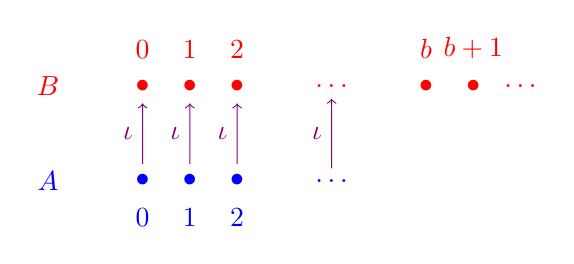
\begin{tikzpicture}[very thick, scale=0.6]
\begin{scope}[color=blue]
\node (A) at (0,0) {$A$};
\node(A0) at (2,0)[label=below:$0$]{$\bullet$};
\node(A1) at (3,0)[label=below:$1$]{$\bullet$};
\node(A2) at (4,0)[label=below:$2$]{$\bullet$};
\node (Adots) at (6,0) {$\ldots$};
\end{scope}
\begin{scope}[color=red]
\node (B) at (0,2) {$B$};
\node(B0) at (2,2)[label=above:$0$]{$\bullet$};
\node(B1) at (3,2)[label=above:$1$]{$\bullet$};
\node(B2) at (4,2)[label=above:$2$]{$\bullet$};
\node (Bdots) at (6,2) {$\ldots$};
\node (b) at (8,2) [label=above:$b$]{$\bullet$};
\node (bsucc) at (9,2) [label=above:$b+1$]{$\bullet$};
\node (Bdots2) at (10,2) {$\ldots$};
\end{scope}
\begin{scope}[color=red!50!blue]
\draw [->,thin] (A0) -- node [auto] {$\iota$} (B0);
\draw [->,thin] (A1) -- node [auto] {$\iota$} (B1);
\draw [->,thin] (A2) -- node [auto] {$\iota$} (B2);
\draw [->,thin] (Adots) -- node [auto] {$\iota$} (Bdots);
\end{scope}
\end{tikzpicture}
   \caption{\textcolor{blue}{$A$} is a sub-segment  of \textcolor{red}{$B$}}
   \label{fig:subsegment}
 \end{figure}




\index{Coq!Commands!Program}

We are now able to build an instance of \texttt{Subsegment}. 

\begin{Coqsrc}
Section Inclusion_ij.

  Variables i j : nat.
  Hypothesis Hij : (i < j)%nat.

   Remark Ltb_ij : Nat.ltb i j.
   Program Definition iota_ij  (alpha: t i) : t j :=  alpha.
 
   Let b : t j := exist _ i Ltb_ij.
   
   Global Instance F_incl_ij  : SubSegment  (FinOrd i) (FinOrd j) b iota_ij.
  (* ... *)

  End Inclusion_ij.

\end{Coqsrc}
         



\begin{remark}
 There is no interesting arihmetic on finite ordinals, since functions like successor, addition, etc.,  cannot be represented in \coq{} as \emph{total} functions.
\end{remark}

\paragraph{Related work}
Finite ordinals are also formalized in MathComp~\cite{SSR}.  See also Adam Chlipala's \emph{CPDT}~\cite{chlipalacpdt2011} for a thorough study of the use of dependent types.

\subsection{The first infinite ordinal : \texorpdfstring{$\omega$}{omega}}

Mathematically speaking, the ordinal $\omega$ is (set-theoretically) considered as the well-ordered set of
natural numbers. 
Every beginner in \coq{} must have seen examples using the type \texttt{nat} of natural numbers. \coq's standard 
library already contains a lot of functions and lemmas on Peano arithmetic. 

In order to build a notation system for $\omega$, we have just to look for lemmas about strict orders and well-foundedness in type \texttt{nat}.

\begin{Coqsrc}
Require Import Arith Compare_dec Lia Simple_LexProd Ordinal_generic.
Import Relations.

Search (@StrictOrder nat).
Search @Nat.compare.
Search (@well_founded nat).
\end{Coqsrc}

\begin{Coqsrc}
Instance Omega : OrdinalNotation Nat.lt_strorder Nat.compare.
Proof.
 split.
 - apply Nat.compare_spec.
 - apply lt_wf.
Qed.
\end{Coqsrc}

We can also prove that any finite ordinal $i$ can be considered as a sub-segment of $\omega$.

\begin{Coqsrc}
Global Instance FinOrd_Omega (i:nat) :
  SubSegment (FinOrd i) Omega i 
             (fun alpha =>  proj1_sig alpha).
\end{Coqsrc}


\subsection{The ordinal \texorpdfstring{$\omega+\omega$}{omega + omega}}

The ordinal $\omega+\omega$ (also known as $\omega\times 2$) may be represented as the concatenation 
of two copies of $\omega$ (Figure~\ref{fig:omega-plus-omega}).

\begin{figure}[h]
   \centering
   \begin{tikzpicture}[very thick, scale=0.5]
\begin{scope}[color=blue]
\node(A0) at (2,0)[label=below:$0$]{$\bullet$};
\node(A1) at (3,0)[label=below:$1$]{$\bullet$};
\node(A2) at (4,0)[label=below:$2$]{$\bullet$};
\node (Adots) at (6,0) {$\ldots$};
\node(An) at (8,0)[label=below:$n$]{$\bullet$};
\node(A2) at (10,0)[label=below:$n+1$]{$\bullet$};
\node (Adots1) at (12,0) {$\ldots$};
\end{scope}
\begin{scope}[color=red]
\node(B0) at (14,0)[label=below:$0$,label=above:$\omega$]{$\bullet$};
\node(B1) at (16,0)[label=below:$1$, label=above:$\omega+1$]{$\bullet$};
\node(B2) at (18,0)[label=below:$2$,label=above:$\omega+2$]{$\bullet$};
\node (Bdots) at (20,0) {$\ldots$};
\node (Bn) at (22,0) [label=below:$p$, label=above:$\omega+p$]{$\bullet$};
\node (Bdots2) at (24,0) {$\ldots$};
\end{scope}
\end{tikzpicture}
   \caption{\textcolor{blue}{$\omega+{\color{red}\omega}$}}
   \label{fig:omega-plus-omega}
 \end{figure}

In \coq{}, we use the disjoint union \texttt{(nat+nat)\%type} for representing the elements of $\omega+\omega$.
The blue ordinals of Figure~\ref{fig:omega-plus-omega} will be represented by terms of the form \texttt{(inl $i$)},
the red ones by \texttt{(inr $j$)}.

\vspace{4pt}
\noindent\emph{From Module~\href{../src/html/hydras.Prelude.Omega_plus_omega.html}{Prelude.Omega\_plus\_omega}}


\begin{Coqsrc}
Declare Scope oo_scope.
Delimit Scope oo_scope with oo.
Open Scope oo_scope.

Definition t := (nat + nat)%type.
Arguments inl  {A B} _.
Arguments inr  {A B} _.
\end{Coqsrc}

The order on type \texttt{t} is already defined in
Library~\href{https://coq.inria.fr/distrib/current/stdlib/Coq.Relations.Relation_Operators.html}{Relations.Relation\_Operators}.

\begin{Coqanswer}
Inductive
le_AsB (A B : Type) (leA : A -> A -> Prop) (leB : B -> B -> Prop)
  : A + B -> A + B -> Prop :=
    le_aa : forall x y : A, leA x y -> le_AsB A B leA leB (inl x) (inl y)
  | le_ab : forall (x : A) (y : B), le_AsB A B leA leB (inl x) (inr y)
  | le_bb : forall x y : B, leB x y -> le_AsB A B leA leB (inr x) (inr y)
\end{Coqanswer}

\begin{Coqsrc}
Definition lt : relation t := le_AsB _ _ Peano.lt Peano.lt.
Infix "<" := lt : oo_scope.

Definition le := clos_refl _ lt.

Infix "<=" := le : oo_scope.
\end{Coqsrc}




\subsubsection{Finite ordinals as members of \texorpdfstring{$\omega+\omega$}{omega+omega}}

It is easy do define a coercion from type \texttt{nat} into our type \texttt{t}.

\begin{Coqsrc}
Definition fin (n:nat) : t := inl n.
Coercion fin : nat >-> t.
\end{Coqsrc}

The range of \texttt{fin} is called the set of \emph{finite} ordinals.


\index{Coq!Techniques!Coercions} 
\begin{remark}
Beware of coercions and notation scopes!

Let us consider the following goal:

\begin{Coqsrc}
 Goal (6 < 8).
 auto with arith.
\end{Coqsrc}


\begin{Coqanswer}
1 subgoal (ID 9)
  
  ============================
  6 < 8
\end{Coqanswer}

Please keep in mind that the current notation scope interprets the infix \texttt{``<''} as the predicate \texttt{Omega\_plus\_omega.lt} and not \texttt{Nat.lt}. More,  the coercion mechanism converts the terms \texttt{6:nat} [resp. \texttt{8:nat} ]
into \texttt{inl 6} [resp. \texttt{inl 8}].  So, the initial goal is correctly interpreted by \coq{}, but not as an inequality between two natural numbers.

Anyway, the initial goal is provable, using \texttt{le\_AsB} first constructor.

\begin{Coqsrc}
  constructor; auto with arith.
Qed.
\end{Coqsrc}

\end{remark}

\subsubsection{Definition of \texorpdfstring{$\omega$}{omega}}

We define $\omega$ as the least ordinal which is larger than any finite ordinal.

\begin{Coqsrc}
 Notation  "'omega'"  := (inr 0) : oo_scope. 
\end{Coqsrc}

\begin{exercise}
Show that, for any $\alpha:t$, $\alpha$ is finite iff $\alpha<\omega$.
\end{exercise}


\subsubsection{Building an instance of OrdinalNotation}

The class \texttt{OrdinalNotation} is parameterized by the strictorder $<$ and a correct comparison function.

First, we prove that \texttt{lt} is an instance of \texttt{StrictOrder}.

\begin{Coqsrc}
Instance lt_strorder : StrictOrder lt.
Qed.
\end{Coqsrc}

Then, we define a comparison function by pattern matching over the sum type $t$.

\begin{Coqsrc}
Definition compare (alpha beta: t) : comparison :=
   match alpha, beta with
     inl _, inr _ => Lt
   | inl n, inl p | inr n, inr p => Nat.compare n p
   | inr _, inl _ => Gt
  end.
\end{Coqsrc}

\begin{Coqsrc}
Compute compare 7 omega.
\end{Coqsrc}

\begin{Coqanswer}
= Lt : comparison
\end{Coqanswer}


\begin{Coqsrc}
Compute compare  (inr 2) 42.
\end{Coqsrc}
 
\begin{Coqanswer}
= Gt : comparison
\end{Coqanswer}

\begin{Coqsrc}
Compute compare (inr 0) omega.  
\end{Coqsrc}
 
 \begin{Coqanswer}
= Eq : comparison
\end{Coqanswer}
 

Correctness of the function \texttt{compare} is asserted by the following lemma:

\begin{Coqsrc}
Lemma compare_correct alpha beta :
    CompareSpec (alpha = beta) (lt alpha beta) (lt beta alpha)
              (compare alpha beta).
\end{Coqsrc}


\begin{todo}
  Well foundedness; instance of OrdinalNotation.
\end{todo}

%%%% ICI %%%%

\subsubsection{Limit and successor ordinals}

The notions of limit and successor are defined in the module 
\href{../src/html/hydras.Prelude.Limits_and_Successors.html}{Prelude.Limits\_and\_Successors} for any instance of
\texttt{StrictOrder}.


\index{Maths!Limit ordinals}

Let $<$ be a strict order on a type $A$ .
We say $x:A$ is an  $\omega$-\emph{limit} of  a sequence $s(i), i\in\mathbb{N}$, if
 if $x$ is [strictly] larger than all the $s(i)$, and for any
$y<x$, $y$ is dominated by at least an element of  the sequence $s$.

\vspace{4pt}

\noindent\emph{From Module~\href{../src/html/hydras.Prelude.Limits_and_Successors.html}{Prelude.Limits\_and\_Successors}}

\begin{Coqsrc}
Definition  Omega_limit
            {A:Type}{lt : relation A}
           {sto : StrictOrder lt} (s: nat -> A) (x:A)  :=
  (forall i: nat, lt (s i) x) /\
  (forall y, lt y  x -> exists i:nat, lt y (s i)).

Definition Limit   {A:Type}{lt : relation A}
           {sto : StrictOrder lt}  (x:A)  :=
  exists s : nat -> A, Omega_limit s x.
 \end{Coqsrc}

Let $x$ and $y$ be two terms of type $A$, we say that \emph{$y$ is a successor of $x$}
if $x<y$ and there is no $z$ strictly greater than $x$ and  strictly less than $y$.



\begin{Coqsrc}
Definition Successor `{lt : relation A}
           {sto : StrictOrder lt} (y x : A):=
  lt x y /\ (forall z,  lt x z -> lt z y -> False).
\end{Coqsrc}


\index{Exercises}

\begin{exercise}
Prove that $\omega$ is the unique   limit ordinal within the notation system for $\omega+\omega$
\emph{(in this precise notation system! In larger segments of 
ordinals, there will be \emph{a lot} of limit ordinals}).
\end{exercise}


\subsection{Computing in \texorpdfstring{$\omega+\omega$}{omega+omega}}

The simple data type we use for representing the ordinals less than $\omega+\omega$ allows us to compute successors, and to decide properties like \texttt{Successor} or \texttt{Limit}. 

\subsubsection{Computing successors}

The following function computes the successor of any ordinal less than $\omega+\omega$, by a simple pattern matching.


\begin{Coqsrc}
Definition succ (alpha : t) := match alpha with
                                 inl i => inl (S i)
                               | inr i => inr (S i)
                               end.

Compute succ omega.
\end{Coqsrc}


\begin{Coqanswer}
  = inr 1
     : nat + nat
\end{Coqanswer}

\begin{Coqsrc}
Lemma lt_succ alpha : alpha < succ alpha.
Proof.
 destruct alpha; constructor; auto with arith. 
Qed.
\end{Coqsrc}

The correctness  of the \texttt{succ} function is asserted by the following lemma.


\begin{Coqsrc}
Lemma Successor_correct alpha beta : Successor beta alpha <-> beta = succ alpha.
\end{Coqsrc}


Being a successor is decidable, thanks to the following boolean function.


\begin{Coqsrc}
Definition succb (alpha: t) := match alpha with
                                   inr (S  _) | inl (S _) => true
                                 | _ => false
                                 end.

Lemma succb_correct alpha : succb alpha <-> exists beta,  alpha = succ beta.
\end{Coqsrc}



\subsubsection{Deciding whether a given ordinal is a limit}

In the same way as successors, one can decide by pattern matching wether a given ordinal (dont' forget less than $\omega+\omega$ !) is a limit.

\begin{Coqsrc}
Definition limitb (alpha : t) := match alpha with
                                     (inr 0) => true
                                   | _ => false
                                   end.

Lemma limitb_correct alpha  : limitb alpha <-> 
                              exists s: nat -> t, Omega_limit s alpha.
\end{Coqsrc}






\begin{todo}
trichotomy zero/succ/limit
boolean functions limitb, succb


\end{todo}
\begin{itemize}
\item $\omega^n$ (for some  integer  $n\geq 2$) : the type of $n$-uples of natural numbers, with the lexicographic product of $n$ copies of \texttt{Nat.lt}.
\item  $\omega^\omega$: the set of nonincreasing sequences of natural numbers, lexicographically ordered (also the set of finite multisets of natural numbers).
\item $\epsilon_0$: The set of terms in Cantor normal form (see Chap.~\ref{chap:T1}).
\item $\Gamma_0$: The set of terms in Veblen normal form.
\end{itemize}



\begin{todo}
The following section has moved from chaper on hydras.
Adapt the redaction to the $\omega^2$ ordinl segment.
\end{todo}


\subsubsection{Lexicographic order on \texorpdfstring{nat*nat}{nat*nat}}
\label{omega2-case}

We  prove now that even the type \texttt{nat * nat}, provided with the lexicographic product of \texttt{(nat,<)} by itself is too simple for proving the termination of all hydra battles. This impossibility result will prevent us from considering measures like the following one:


  \begin{Coqsrc}
  Let m h = (height h, hsize h).
  \end{Coqsrc}

The proof we are going to develop has exactly the same structure as in Section~\ref{sect:omega:case}


previous one. Nevertheless, the proof of technical  lemmas is a little more complex, due to 
 the structure of the lexicographic order on $\mathbb{N}\times\mathbb{N}$. 
Consider for instance that there exists an infinite number of pairs between
$(1,0)$ and $(2,0)$.


\begin{remark}
  The order structure we consider in this section is also known as the ordinal
  $\omega^2$. We identify any pair $(i,j)\in \mathbb{N}\times\mathbb{N}$ with the ordinal $\omega\times i + j$. Thus the three kinds of ordinals in $\omega^2$
  are represented as follows:
  \begin{description}
  \item[null ordinal] : the pair $(0,0)$
  \item[successor ordinal] : any pair $(i,j)$ where $j>0$
  \item[limit ordinal] : any pair $(i,0)$ where $i>0$
  \end{description}
\end{remark}

The detailed  proof script is in the file \url{../src/html/hydras.Hydra.Omega2_Small.html}.

\subsubsection{Preliminaries}
Let us assume there is a variant from \texttt{Hydra} into \texttt{nat*nat} (with the
   lexicographic ordering)  for proving the   termination of all hydra battles.

\vspace{4pt}
\emph{From Module~\href{../src/html/hydras.Hydra.Omega2_Small.html}{Hydra.Omega2\_Small}}


\begin{Coqsrc}
  Section Impossibility_Proof.
  
  Let t := (nat * nat)%type. 

  (** non-dependent lexicographic strict ordering on nat*nat *)
  
  Let lt2 : relation t := lexico Peano.lt Peano.lt.

  Infix "<" := lt2.
  
  (** reflexive closure of lt2 *)
  Let le2 := clos_refl _ lt2.
  Infix "<=" := le2.

  Variable m : Hydra -> t.
  
  Context (Hvar : Hvariant lt2_wf free m).
\end{Coqsrc}


Let us follow the same pattern as in Sect.~\ref{omega-case}.
First, we define an injection from type \texttt{t} into \texttt{Hydra}.
We associate with any pair $(i,j)$ the hydra with $i$ branches of length $2$ and
$j$ branches of length $1$.

%% revenir ici

\vspace{4pt}
\emph{From Module ~\href{../src/html/hydras.Hydra.Omega2_Small.html\#iota}{Hydra.Omega2\_Small}}

\begin{Coqsrc}
  Let iota (p: t) := 
    node (hcons_mult (hyd1 head) (fst p)
                     (hcons_mult head (snd p) hnil)).
\end{Coqsrc}

For instance, Figure~\vref{fig:essai2} shows the hydra associated to the pair
$(3,5)$. 

\begin{figure}[htb]
\centering
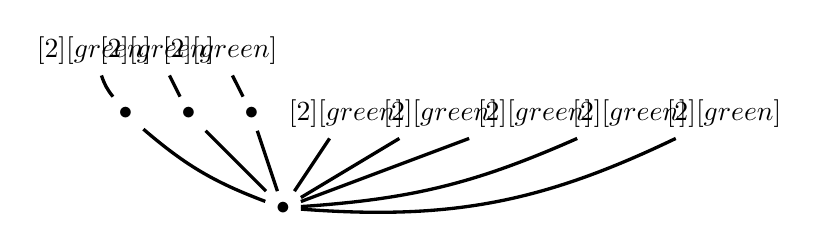
\begin{tikzpicture}[very thick, scale=0.4]
\node (foot) at (6,0) {$\bullet$};
\node (N1) at (1,3) {$\bullet$};
\node (N2) at (3,3) {$\bullet$};
\node (N3) at (5,3) {$\bullet$};
\node (N4) at (8,3) {$\Smiley[2][green]$};
\node (N5) at (11,3) {$\Smiley[2][green]$};
\node (N6) at (14,3) {$\Smiley[2][green]$};
\node (N7) at (17,3){$\Smiley[2][green]$};
\node (N8) at (20,3){$\Smiley[2][green]$};
\node  (N9) at (0,5) {$\Smiley[2][green]$};
\node (N10) at (2,5) {$\Smiley[2][green]$};
\node (N11) at (4,5) {$\Smiley[2][green]$};
\draw (foot) to [bend left=10] (N1);
\draw (foot) -- (N2);
\draw (foot) -- (N3);
\draw (foot) -- (N4);
\draw (foot) -- (N5);
\draw (foot) -- (N6);
\draw (foot) to [bend right=10] (N7);
\draw (foot) to [bend right=15] (N8);
\draw (N1) to [bend left=10] (N9);
\draw (N2) -- (N10);
\draw (N3) -- (N11);
\end{tikzpicture}
\caption{\label{fig:essai2}
The hydra $\iota(3,5)$}
\end{figure}




Like in Sect.~\ref{omega-case}, we build a hydra out of the range of \texttt{iota} (represented in Fig.~\vref{fig:h-omega2-small}).

\begin{figure}[htb]
\centering
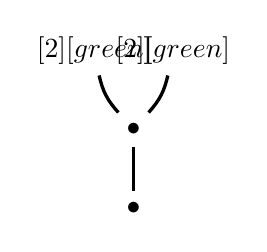
\begin{tikzpicture}[very thick, scale=0.5]
\node (foot) at (2,0) {$\bullet$};
\node (N1) at (2,2) {$\bullet$};
\node (N2) at (3,4) {$\Smiley[2][green]$};
\node (N3) at (1,4) {$\Smiley[2][green]$};
\draw (foot) -- (N1);
\draw (N1) to [bend right =15] (N2);
\draw (N1) to  [bend left=15](N3);
\end{tikzpicture}
\caption{\label{fig:h-omega2-small}}
 The hydra \texttt{big\_h}.
\end{figure}
\begin{Coqsrc}
   Let big_h := hyd1 (hyd2 head head).  
 \end{Coqsrc}
 
 In a second step, we build a ``smaller'' hydra.
 
\begin{Coqsrc}
   Let small_h := iota (m big_h).
\end{Coqsrc}

Like in Sect.~\ref{omega-case}, we prove the double inequality \texttt{m big\_h <= m small\_h < m big\_h}, which is impossible.

\subsubsection{Proof of the inequality \texttt{m small\_h < m big\_h}}

For proving the inequality  \texttt{m\_lt: m small\_h < m big\_h}, it suffices to
build a fight transforming \texttt{big\_h} into \texttt{small\_h}.

First we prove that \texttt{small\_h} is reachable from \texttt{big\_h} in one or two steps. Let us decompose \texttt{m big\_h}
into the pair $(i,j)$.
If $j=0$, then one round suffices to transform \texttt{big\_h} into $\iota(i,j)$.
If $j>0$, then a first round transforms \texttt{big\_h} into $\iota(i+1,0)$ and a second round into $\iota(i,j)$. So, we have the folowing result.

\begin{Coqsrc}
 Lemma big_to_small: big_h -+-> small_h.
\end{Coqsrc}

Since $m$ is a variant, we infer the following inequality:

\begin{Coqsrc}
Corollary m_lt : m small_h < m big_h.
\end{Coqsrc}


\subsubsection{Proof of the inequality \texttt{m big\_h <= m small\_h} }


The proof of the inequality \texttt{m big\_h <= m small\_h} is quite more complex than in Sect~\ref{omega-case}.  If we consider some pair $(i,j)$, where $i>0$, there exists an infinite number of
pairs stricly less than $(i,j)$, and there exists an infinite number of battles that start from
$\iota(i,j)$. In effect, at any configuration $\iota(k,0)$, the hydra can freely chose any replication number. Intuitively, the measure of such a hydra must be large enough for taking into account
all the possible battles issued from that hydra.
Let us give more technical details.

\begin{itemize}
\item The proof of the lemma \texttt{m\_ge : forall p : t,   p <= m (iota p)} uses well-founded induction on $p$, and not structural induction on natural numbers

\item For any pair $p$, we have to distinguish between three cases, according to the value of $p$'s components.
  \begin{itemize}
  \item $p=(0,0)$
  \item $p=(i,0)$, where $i>0$\,: $p$ corresponds to a limit ordinal
  \item $p=(i,j)$, where $j>0$\,: $p$ is the successor of $(i,j-1)$.
  \end{itemize}
\end{itemize}

Before starting the proof, we have to express the notion of \emph{limit} in terms of
least upper bounds, through the following logical equivalence.

\vspace{4pt}
\emph{From Module ~\href{../src/html/hydras.Hydra.Omega2_Small.html\#limit_is_lub}{Hydra.Omega2\_Small.v}}.

\begin{Coqsrc}
Lemma limit_is_lub : forall i p, 
   (forall j, (i,j) < p) <-> (S i, 0) <= p.  
\end{Coqsrc}

Let us define the notion of elementary ``step'' of decreasing sequences in
\texttt{t}


\begin{Coqsrc}
Inductive step : t -> t -> Prop :=
| succ_step : forall i j,  step (i, S j) (i, j)
| limit_step : forall i j, step (S i, 0) (i, j).
\end{Coqsrc}

The following lemma establishes a correspondance between the relation
\texttt{step} and hydra fights.

\begin{Coqsrc}
Lemma step_to_fight : forall p q, step p q -> iota p -+-> iota q.
\end{Coqsrc}

\index{Maths!Transfinite induction}

Thus, starting from any inequality $q < p$ on type \texttt{t}, we can build 
by transfinite induction over \texttt{p} a fight 
that transforms the hydra $\iota(p)$ into $\iota(q)$.

\vspace{4pt}
\emph{From Module~\href{../src/html/hydras.Hydra.Omega2_Small.html\#m_ge}{Hydra.Omega2\_Small}}

\begin{Coqsrc}
Lemma m_ge : forall p : t,   p <= m (iota p).
Proof.
  intro p ; pattern p;
    apply  well_founded_induction with 
               (R := lt2) (1:= wf_lexico lt_wf lt_wf);
     intros (i,j) IHij (* rest of proof skipped *)
\end{Coqsrc}

\begin{Coqanswer}
  i, j : nat
  IHij : forall y : t, y < (i, j) -> y <= m (iota y)
  ============================
  (i, j) <= m (iota (i, j)) 
\end{Coqanswer}


Then we have  three cases to consider, according to the values of $i$ and $j$.
\begin{itemize}
\item If $p=(0,0)$ then obviously, $\iota(p)\geq p = (0,0)$
\item If  $p=(i+1,0)$ for some $i\in\mathbb{N}$, we
 remark  that $p$ is strictly greater than any pair $ (i, j)$, where $j$ 
is any natural number.

Applying the battle rules, for any $j$, we have $\iota(i+1,j)  {\round} \iota(i, j) $, thus $m(\iota(p)) > m(\iota(i,j)$ since  $m$ is assumed to be a variant.

Applying the induction hypothesis, we get the inequality
 $ m(\iota(i,j)) \geq (i,j)$ for any $j$. 

Thus, $m(\iota(p)) > (i,j)$ for any $j$.
Applying the lemma \texttt{limit\_is\_lub}, we get  the inequality
$\iota(i+1,0)\geq (i+1,0)$

\item If $p=(i,j+1)$ with $j\in\mathbb{N}$, we have  $\iota(p)  {\round} \iota(i, j) $,
hence $m(\iota(p))> m(\iota(i,j)) \geq (i,j)$, thus $m(\iota(p))\geq (i,j+1)=p$

\end{itemize}

\subsubsection{End of the proof}

Since $<$ is a strict order (irreflexive  and transitive) on \texttt{nat*nat}, we can conclude that there is no
variant for termination on the lexicographic square of $(\mathbb{N},<)$.

\begin{enumerate}
\item From \texttt{m\_lt}, we infer the strict inequality 
\texttt{m small\_h < m big\_h}
\item from \texttt{m\_ge}, we get \texttt{m big\_h <= m (iota (m big\_h)) = m small\_h} 
\end{enumerate}


\vspace{4pt}
\emph{From Module~\href{../src/html/hydras.Hydra.Omega2_Small.html}{Hydra.Omega2\_Small}}

\begin{Coqsrc}
Theorem Impossible : False.
Proof.
  destruct (StrictOrder_Irreflexive  (m big_h)).
  apply le2_lt2_trans with (m small_h).
  -  unfold small_h;  apply m_ge.
  -  apply m_lt. 
Qed. 

End Impossibility_Proof.
\end{Coqsrc}

\index{Exercises}

\begin{exercise}
Prove that there exists no variant $m$ from \texttt{Hydra} into \texttt{nat*nat} for proving
    the  termination of all \emph{standard} battles.
\end{exercise}



\begin{remark}
In Chapter~\ref{ks-chapter}, we will prove a much more general  theorem
than the two previous results about $\mathbb{N}$ and $\mathbb{N}\times\mathbb{N}$. The proof of that general  result will share the same structure, but will 
require a lot of technical results. 
\end{remark}

\begin{exercise}

\label{sec:orgheadline63}
Write \emph{direct} proofs ({i.e.},  without applying the result and tools of Chap.~\ref{ks-chapter}) that the following data structures  are too simple for defining a variant for any hydra battle.

\begin{itemize}
\item  $\omega^n$ : the set of all $n$-uples of natural numbers, ordered  by 
  lexicographic ordering
\item  $\omega^\omega$: the set of all decreasing sequences (with respect to $\le$)  of natural numbers, ordered by lexicographic ordering on lists.

For instance , the sequence $\langle 4,4,2 \rangle$ is strictly greater than 
$\langle 4,3,3,3,3,3,3,2,2,2 \rangle$.
\end{itemize}

  
\end{exercise}


